\documentclass[letterpaper,10pt]{article}
\usepackage{fullpage}
\usepackage{subfigure}
\usepackage{textcomp}
\usepackage{times}
\usepackage{cite}
\usepackage[small,compact]{titlesec}
\usepackage{caption}
\usepackage{fancyvrb}
\usepackage{moreverb}
\usepackage{graphicx}
\usepackage{hyperref}
\usepackage{multicol}
\usepackage{verbatim}

\newcommand{\squishlist}{\begin{list}{$\bullet$}
  {\setlength{\itemsep}{0pt}
    \setlength{\parsep}{3pt}
    \setlength{\topsep}{3pt}
    \setlength{\partopsep}{0pt}
    \setlength{\leftmargin}{1.5em}
    \setlength{\labelwidth}{1em}
    \setlength{\labelsep}{0.5em}
  } }

\newcommand{\squishend}{\end{list}}

\makeatletter
\newenvironment{tablehere}
{\def\@captype{table}}
{}
\newenvironment{figurehere}
{\def\@captype{figure}}
{}
\makeatother

\title{My Other Computer is your GPU:\\
System-Centric CUDA Threat Modeling with CUBAR}
\author{Nick Black and Jason Rodzik\\
CS8803SS Project, Spring 2010}
\date{}

\begin{document}
\maketitle

\begin{quotation}\scriptsize\textit{``The charm of history and its enigmatic lesson consist in the fact that, from age to age, nothing changes and yet everything is completely different.''}

\hfill---Aldous Huxley \end{quotation}

\begin{abstract}
\textbf{Heterogeneous computing has definitely arrived, and graphics processing
units (GPUs) in the millions are employed worldwide. History has shown newly
programmable domains to be rapidly subjected (and often found vulnerable) to
attacks of the past. We enumerate a system-centric threat model using Microsoft's
STRIDE process\cite{stride}. We then describe an active general purpose
programming system, NVIDIA's Compute Unified Device Architecture
(CUDA) \footnote{NVIDIA, CUDA, and GeForce are trademarks or registered trademarks of the NVIDIA Corporation.},
and explore the threat space. We derive
and describe previously-undisclosed memory protection and translation processes
in CUDA, successfully mount several attacks on the CUDA system, and identify
numerous directions for future work. Our CUBAR suite of tools, especially \texttt{cudash}
(the CUDA Shell), form a solid platform for research to come.}

\end{abstract}
\begin{multicols}{2}
\section{Introduction}
Within modern desktops, high-performance workstations, and even laptops there
exist sources of tremendous computing power: programmable, massively parallel graphics cards.
The hundreds of simple in-order cores found on recent NVIDIA and ATI hardware provide many more peak FLOPS than the x86 processor packages with
which they're commonly coupled.
Devices such as NVIDIA's Tesla\texttrademark{} have already traded video outputs for onboard memory, giving rise to ``desktop
supercomputing.'' Those who would fully utilize their machines can
no more ignore heterogeneous processing than multiple cores or SIMD\@.

But is it safe? GPUs have traditionally accelerated
single-instance, interactive tasks (such as video games and CAD) and
decomposable, compute-bound tasks (such as batch rendering) for which a
deinterleaved schedule is optimal. Hardware facilities for the support of
multiple threads or processes are primitive at best. When the GPU was limited to
blitting, fogging, and anti-aliasing framebuffers, minimal isolation and
assurance capabilities were tolerable. Compromises of scientific data,
cryptographic materials and SCADA systems are rather more serious, yet these
precise applications drive the adoption of GPGPU programming. 

We explored CUDA 3.0 on a 2.6.34-rc2 Linux kernel, using version 195.36.15
of the CUDA software. Hardware included a GTS 360M, a GeForce 8400 GS, and a
GT 9600. Our source code can be found on GitHub\footnote{\url{http://github.com/dankamongmen/wdp/tree/master/cs8803ss-project/}}.

\section{An overview of CUDA}
A GPU-accelerated CUDA application on Linux adds four component parts to
a typical process:
\squishlist
\item A ``fat binary'' containing host and guest object code, typically x86 and PTX\cite{ptxguide}.
Note that PTX is a mere intermediate representation, converted to the native
CUBIN format at runtime.
\item The CUDA userspace library \texttt{libcuda.so}. This closed-source archive
provides an interface to the NVIDIA driver, and management of a CUDA instance.
\item The NVIDIA driver \texttt{nvidia.ko}. This closed-source module handles
\texttt{ioctl}s issued by \texttt{libcuda.so}.
\item The hardware, controlled by registers and memory-mapped IO.
\squishend
No complete open-source CUDA solution yet exists.

The CUDA language is an extension of C++, designed for compilation with NVIDIA's \texttt{nvcc}\cite{nvcc}
toolchain. NVIDIA states that a given device supports multiple host threads,
but that a given host thread can control only one device. Data must either be
explicitly copied between system and video RAM or, on devices of Compute Capability
1.2 or higher, restricted to shared memory maps\cite{cudaguide}. GPU processes
(``kernels'') can be launched asynchronously, though (until Compute Capability
2.0) only one kernel can be executed at a time by a given device.

CUDA supports numerous memory ``spaces'', selected via PTX affixes (until the
advent of unified addressing in Compute Capability 2.0, presumably effected via
memory translation). Spaces differ according to caching, method of
initialization, visibility across the device's multiprocessors, and mutability.
Official documentation does not address memory protection or translation.

CUDA kernels are typically distributed as JIT-friendly PTX binaries\cite{kerr},
an intermediate representation suitable for all NVIDIA hardware. Upon being
loaded onto the card, dynamic compilation\footnote{Likely performed in the
driver, not the hardware, though we have not yet verified this.} is performed,
resulting in a locally-optimized CUBIN blob. These blobs are dispatched to
Streaming Multiprocessors across the card, all of which share a common memory.
A given system thread can use only one device at a time, but a device may be
used by more than one system thread.

In our case, the \texttt{nvidia.ko} kernel module and \texttt{libcuda.so}
library weigh in at thirteen and seven megabytes respectively. We can assume
them to contain substantial logic. Ultimately, some of our questions can be
answered only via analysis of these binaries. This is a matter of some importance
for open source projects seeking to duplicate CUDA functionality, such as the
Nouveau Project and \texttt{libcudest}\cite{libcudest}.

\subsection{Existing controls}
The \texttt{/dev/nvidiaX} device nodes control access to the CUDA hardware and
kernelspace component. Under the standard Linux security model, these
will be restricted via 0660 permissions to a group (typically \texttt{video}).
Membership in the owning group is thus necessary and sufficient to satisfy the
operating system. \texttt{strace} output for CUDA applications, along with
NVIDIA's \texttt{nvidia-smi} device configuration program, show use of the
\texttt{geteuid} system call, but no further access controls are exported to
the user.

\section{Threat model}
Well-known threat taxonomies include the ``CIA Triad'' (extended by the
``Parkerian Hexad\cite{sechandbook}'') and Microsoft's STRIDE\@. The latter, developed as part of
Microsoft's Secure Product Lifecycle, is designed for system-centric threat
modeling and suitable for our purposes. We assume that an attacker has access
to the NVIDIA device node(s) (by default, \texttt{/dev/nvidiaX}); such privileges
are necessary to compute on the device, and thus a safe assumption. Escalation
to device access is an attack on the operating system's access control, and
outside the scope of this paper.

We seek to answer the following questions, for machines with one or more CUDA-capable
cards:
\subsection{Spoofing}
\squishlist
\item Is it possible for one CUDA kernel to pre\"empt data copies requested
from another?
\squishend
\subsection{Tampering}
\squishlist
\item Can one CUDA kernel manipulate another's data set?
\item Is it possible to construct a debugging environment around other CUDA kernels?
\item Can a CUDA kernel modify the active display?
\item Is it possible to pervert compilation processes, either \texttt{nvcc} or JIT?
\squishend
\subsection{Repudiation}
\squishlist
\item Can a CUDA kernel disassociate itself from the system process which spawned it?
\item Can a CUDA kernel spawn new CUDA kernels?
\item What forensic data, if any, is created as a result of CUDA computing?
\squishend
\subsection{Information disclosure}
\squishlist
\item Can a CUDA kernel read another kernel's data set? Need they be simultaneously
scheduled for this to occur?
\item Is it possible to read another CUDA kernel's code, even if it cannot be
controlled?
\item Is it possible to read the system memory of another CUDA application via
calls through the CUDA intermediary?
\item Is it possible to reconstruct the system's video channel from an arbitrary
CUDA kernel? What about textures?
\squishend
\subsection{Denial of service}
\squishlist
\item Can a CUDA kernel monopolize resources in the face of competitors?
\item Can a CUDA kernel prevent another from being controlled, or executing
data transfers to or from the system?
\item Can a CUDA kernel deny resources beyond the GPU\@?
\squishend
\subsection{Escalation of privilege}
\squishlist
\item Might the driver be exploited, allowing arbitrary ring 0 code to run?
\item If it is possible to return doppelg\"anger data, might it be leveraged
to attack (and hopefully exploit) system-side processes?
\item Is it possible to arbitrarily (i.e.\ without exploitation) manipulate
another CUDA kernel's code? Is it possible to construct a CUDA virus?
\item Is it possible to arbitrarily (i.e.\ without exploitation) manipulate a
system process's code maps from a CUDA kernel?
\squishend

\section{Methodology}
Some of the questions asked by our threat model can be answered via simple
experiments (others, such as whether the driver might be exploited, are
essentially undecidable). Describing the internal mechanisms implementing these
externally-visible properties generally requires disassembly, and is the object
of further work.

It is first necessary to develop a model of memory protection, multiple user
contexts, and memory layout in CUDA. Few details have been made public
regarding these topics; what public knowledge exists takes the form of
scattered fora posts, Wikis\cite{nouveaucuda}, and mailing lists. Foremost among these is memory
protection; a trusted multiprocess computing base cannot be constructed in its
absence. Memory protection for host accesses of the GPU could be implemented at
three levels, each more effective than the last:
\squishlist
\item the proprietary CUDA and OpenGL libaries,
\item the proprietary \texttt{nvidia.ko} kernel driver, and
\item on the hardware itself.
\squishend
Userspace protection can likely be thwarted by userspace code, whereas
protection implemented within the kernel module ought be secure against
all but ring 0 operations (recall that our threat model does not assume access
to ring 0). It is unlikely that protection on the card itself can be generally
circumvented. Furthermore, this is the only place to protect memory from CUDA
kernels.

As an example of the futility of userspace protection, we were trivially able
(contrary to NVIDIA documentation) to control multiple devices from a single
host thread. Use of the \texttt{ltrace} library call tracer indicated CUDA
context association to be performed via \texttt{pthread\_key\_t} thread-specific
data. By interpositioning ourselves between the binary and \texttt{libpthread.so},
we implemented our own context-multiplexing.

The PTX Reference provides some details. Load and store instructions require a ``state space''
modifier in addition to an address. General-purpose registers (\texttt{r0}--\texttt{r127}) are
indexed via 7-bit immediates. Global memory, accessed via one of 16 linear ranges
of up to 4GB each (\texttt{g0}--\texttt{g15}), is addressed via the
contents of a 32-bit general purpose register\footnote{Platforms such as the Tesla\textsuperscript{\texttrademark} C1060 provide the
full 4GB of accessible memory. Compute Capability 2.0 unifies addressing
and extends addresses to 64 bits. 40 physical bits are currently
supported for up to 1TB of RAM.}. Constant memory is referenced through one of 16 linear ranges of up to
64KB each (\texttt{c0}--\texttt{c15}), as is a block-shared region of up to 16KB.
Per-thread local memory, an abstraction atop the global memory, performs
address translation based on block and thread indices.
% Other state spaces are addressed
%via the sum of an address register (\texttt{a0}--\texttt{a7}) and an immediate offset.
\subsection{Tools}
Beyond the basic toolchain, we made use of:
\squishlist
\item \texttt{vbtracetool}\cite{vbtrace} to dump video BIOS,
\item \texttt{cuda-gdb}\cite{cudagdb} to debug CUDA programs,
\item \texttt{strace}\cite{stracecode} to track system calls,
\item \texttt{nv50dis}\cite{nv50dis} to disassemble nv50 binaries,
\item \texttt{nvtrace}\cite{nvtrace} to decipher \texttt{ioctl}s issued to the NVIDIA proprietary driver, and
\item the Linux kernel's MMIOTrace\cite{mmiotrace} infrastructure to track memory-mapped I/O operations.
\squishend
We then developed some tools:
\squishlist
\item \texttt{cudadump} (and its helper binary, \texttt{cudaranger}) to
discover readable regions in a given virtual memory,
\item \texttt{cudash}, the CUDA Shell, to perform close-in experiments and
prototype attacks, and
\item \texttt{cudabounder}, \texttt{cudaminimal}, \texttt{cudapinner}, \texttt{cudaquirky}, \texttt{cudaspawner}, and \texttt{cudastuffer}, a series of single-purpose attack tools.
\squishend
\vfill
\begin{figurehere}
\centering
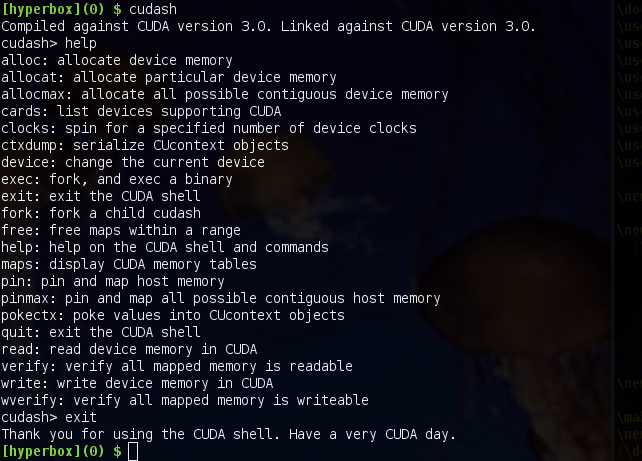
\includegraphics[width=\columnwidth]{texobjs/cudash-help.png}
\end{figurehere}
\section{Attacking CUDA (A dialogue)}
We now move beyond the realm of the documented.
\subsection{Von Neumann or Harvard architecture?}
\textit{CUDA appears to be a Harvard architecture.} Kernels do occupy
video memory, as can be verified by dumping the video RAM. We assert that, by
default, a given kernel's code is neither readable nor writeable using
the global state space. The former was tested by verifying that global state
spaces checksummed to the same value over distinct, subsequent kernels (all of
which operated strictly on the shared memory space). The latter was tested by
reversing all possible bits in the global memory space, and then performing a
series of calculations. It is possible that undocumented opcodes can retrieve
or modify code.

This is puzzling: the Harvard architecture's primary advantage is the ability
to fetch instructions and data into the CPU simultaneously. We suggest that
coherence simplification, combined with the weak memory assurances of the global
memory space, motivated this solution.
\subsection{Is virtual memory implemented?}
\textit{CUDA implements virtual memories.} We conclusively demonstrated this
by examining allocation results in multiple concurrent CUDA contexts. Returned
device pointers are equivalent for equivalent allocations in multiple contexts.
Allocations begin at 0x101000, honor a minimum alignment of 256 bytes (larger
alignments are honored for very large allocations), and otherwise move
contiguously through memory. Freed regions can be reclaimed. This suggests
multilevel memory allocation, split between user and kernelspace.

Physical memory cannot be aliased or oversubscribed; multiple contexts'
maximum allocations cannot add up to more than a single context's maximum
possible allocations.
\subsection{Does memory protection exist?}
\textit{CUDA enforces memory protection in hardware.} Use of a general-purpose,
word-sized register when referencing the global space means kernels' memory
accesses cannot be preverified, and the possibility of software-assisted memory
protection can be eliminated by analyzing details of memory transactions
relative to the device clock\cite{microbenchmarks}. The use of two-level TLBs
has been illustrated in previous work\cite{demmel}. We verified memory
protection to be effective beyond the combined capacities of the TLBs, and
note a L2 TLB miss to be only about half again as expensive as a L2 TLB hit.
Thus we assert that memory protection is performed independently of, and in
parallel with, address translation. This requires virtual- (and thus per-context)
indexing; together with a memory protection granularity (1MB) distinct from
either TLB size (4KB and 8MB), we consider this to imply a backing store in
video RAM, and that memory protection is a single bit per entry.

Members of the \texttt{cuMemset*()} family of functions, when given an invalid device address,
neither return an error nor segfault. Instead, later context functions return
a 700 (previous kernel failed) error. This strongly suggests that memory
protection is \textit{not} modeled in software. Further research, especially
involving shared, pinned maps, ought investigate this further.
\subsection{Does memory protection incorporate contexts?}
\textit{CUDA hardware considers contexts.} To ensure that memory isolation
was not being implemented purely through translation, we allocated a large
region of memory in one context, and operated on it. We then ensured that a
distinct, simultaneous context failed accessing any possible address. This
suggests that some manner of unforgeable \textit{capability}\cite{capability}
lies at the heart of a CUDA context.

Here, we make a controversial conjecture: these capabilities \textit{can}
be forged. We draw this conclusion from the interaction of CUDA and the \texttt{fork}
system call. A CUDA application's system resources are wholly accessible by a
child process up until being unmapped via \texttt{exec} or some other system call.
Furthermore, we verified allocations or kernels executed in either process following the
\texttt{fork} to be visible in the other. We were unable to forge a context,
but think it likely that disassembly of the CUDA stack would make a method plain.
It is likely that some memory-mapped I/O is involved independent of the context
object itself; \texttt{fork}, which preserves maps, thus naturally facilitates
context-forging (the \texttt{/dev/nvidiaX} maps, as can be seen in \texttt{/proc/X/maps},
are mapped \texttt{MAP\_SHARED} and thus not subject to Copy-on-Write behavior).
\subsection{Is memory scrubbed between kernels?}
\textit{CUDA does not scrub memory.} This was demonstrated conclusively by
verifying that a large (8MB) random string could be recovered, contiguously and
in its entirety, by a subsequent kernel. It was not possible to determine
whether code regions were scrubbed, since CUDA does not support indirect
branches. The \texttt{cudawrapper}\cite{cudawrapper} tool has been
developed to provide scrubbing, but the authors consider it highly dubious
that this userspace wrapper could successfully deal with an uncatchable signal.
\subsection{Can kernels disassociate from processes?}
\textit{The CUDA kernelspace tracks processes.} This was conclusively
demonstrated by sending SIGKILL signals to CUDA processes after they had
performed large allocations and launched intense, long-running kernels. There
was no opportunity for userspace code to run, yet these resources were properly
freed upon process termination.
\subsection{Can a kernel fork?}
\textit{CUDA kernels do not appear capable of forking}. A \textit{primum movens} in the
form of a host-system CPU is required to launch a CUDA kernel. The kernel-launching
interface must, therefore, be visible to the host. There is no compelling reason to
then duplicate this interface within the GPU.

Until the mechanism used to launch a kernel is known, however, we cannot be sure
that the following loophole does not exist: devices of Compute Capability 1.2 or higher
can map host memory into a context's address space. If kernels are launched
entirely via memory-mapped I/O transactions, and the map through which this is
done is mapped again, this time into shared memory, device code might be able
to manipulate the device. At this point, all bets are off.
\subsection{Does CUDA produce forensics?}
\textit{CUDA provides insufficient forensic data.} CUDA kernels are not tied
into the process accounting mechanism. Exceptions are delivered to klogd, but
rate-limited within the kernel itself; it would be trivial to hide a meaningful
exception behind a flurry of meaningless ones, as this policy cannot be
overridden. No system exists to log who ran what kernel, or for how long.

The \texttt{nvidia-smi} tool claims to decode and report exceptions as stored
in a hardware buffer, similar to the Machine Check Exception registers of x86.
We were not, however, able to generate any informative output using \texttt{nvidia-smi}.
\subsection{Does CUDA enforce resource limits?}
\textit{CUDA provides no resource limits.} UNIX provides a rich set of resource
limits via the \texttt{rlimit} mechanism. These are just as important for
protecting against programming errors as assuring fair resource distribution.
CUDA neither honors the existing infrastructure, nor provides any of its own.
Device memory allocations do not count against \texttt{RLIMIT\_AS}, kernel
execution time does not count against \texttt{RLIMIT\_CPU}, and executing
kernels are not bounded by \texttt{RLIMIT\_NPROC}.
\subsection{Can CUDA deny access to system resources?}
\textit{CUDA allows system RAM to be monopolized.} Devices of Compute Capability
1.2 or higher support mapping host memory into a device's address space. For this
to be done, the memory must be \textit{pinned} (also known as \textit{locked}), and
thus protected against swapping. Since this makes physical memory unusable by the
rest of the system, memory pinning is strictly limited using the \texttt{RLIMIT\_MEMLOCK}
limit (the default value on Debian Linux is 64KB). CUDA, allocating system memory
from within kernelspace, does not honor this limit. This more than once resulted in
Linux's ``OOM (Out-of-Memory) killer'' delivering SIGKILL to Firefox or even sshd
processes during testing.
\subsection{Any miscellaneous security issues?}
\textit{CUDA introduces sundry security issues.} The CUDA installer (which
must be run as root throughout) contacts an anonymous FTP server to check for
updated versions of the driver. This is open to any number of classic man-in-the-middle
attacks, leaving the user open to trojans. Even if the download was signed,
running the downloader as root leaves the system vulnerable to user agent
exploits.

The \texttt{nvcc} compiler does not support a \texttt{-pipe} option ala GCC,
instead forcing use of temporary files for multiphase operations. The temporary
names used are wholly predictable, suggesting vulnerability to a class of
symlink attack. Successfully attacking this scheme via named FIFOs, and thus
providing a \texttt{-pipe} capability for \texttt{nvcc}, is left as an exercise
for the reader.

The ability of any CUDA application to monopolize device memory facilitates
``use-of-NULL'' attacks throughout the graphics stack, much like those which have plagued
the Linux kernel in 2009 and 2010. Below, see two corrupted displays. It is doubtful that
our CUDA application actively molested the display, since it simply allocated
device memory; more likely, the programs ignored some allocation failure.

Behold the grim visage of undefined behavior:

\begin{figurehere}
\centering
\subfigure[Corrupted AA]
{
    \label{fig:sub:a}
    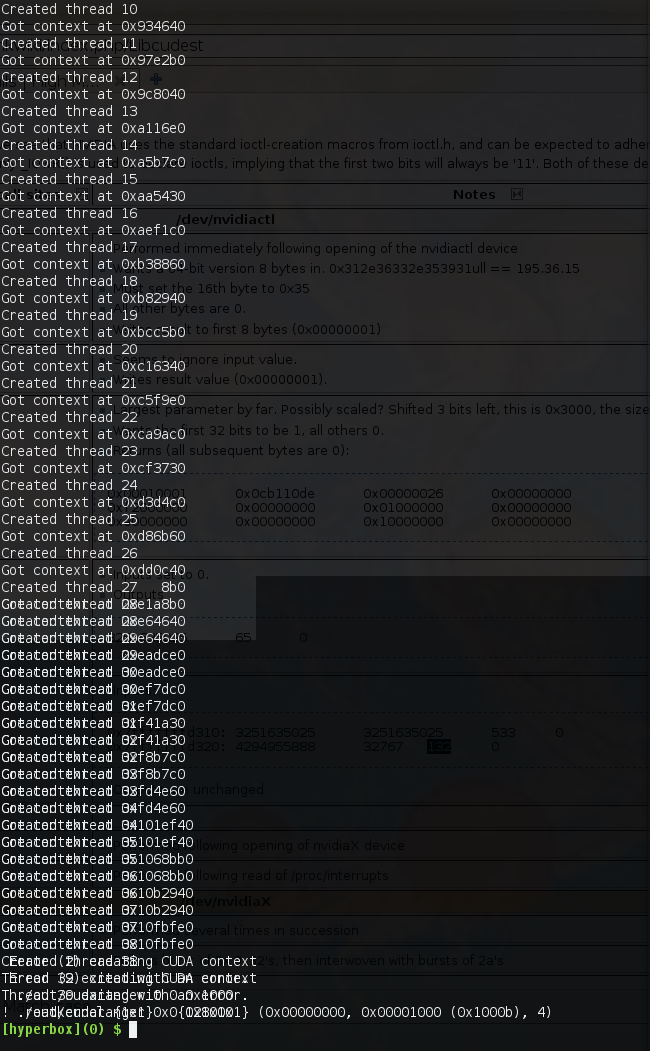
\includegraphics[width=4cm,height=2.25cm]{texobjs/fuckedterminal.png}
}
\subfigure[Pixellated VDPAU]
{
    \label{fig:sub:b}
    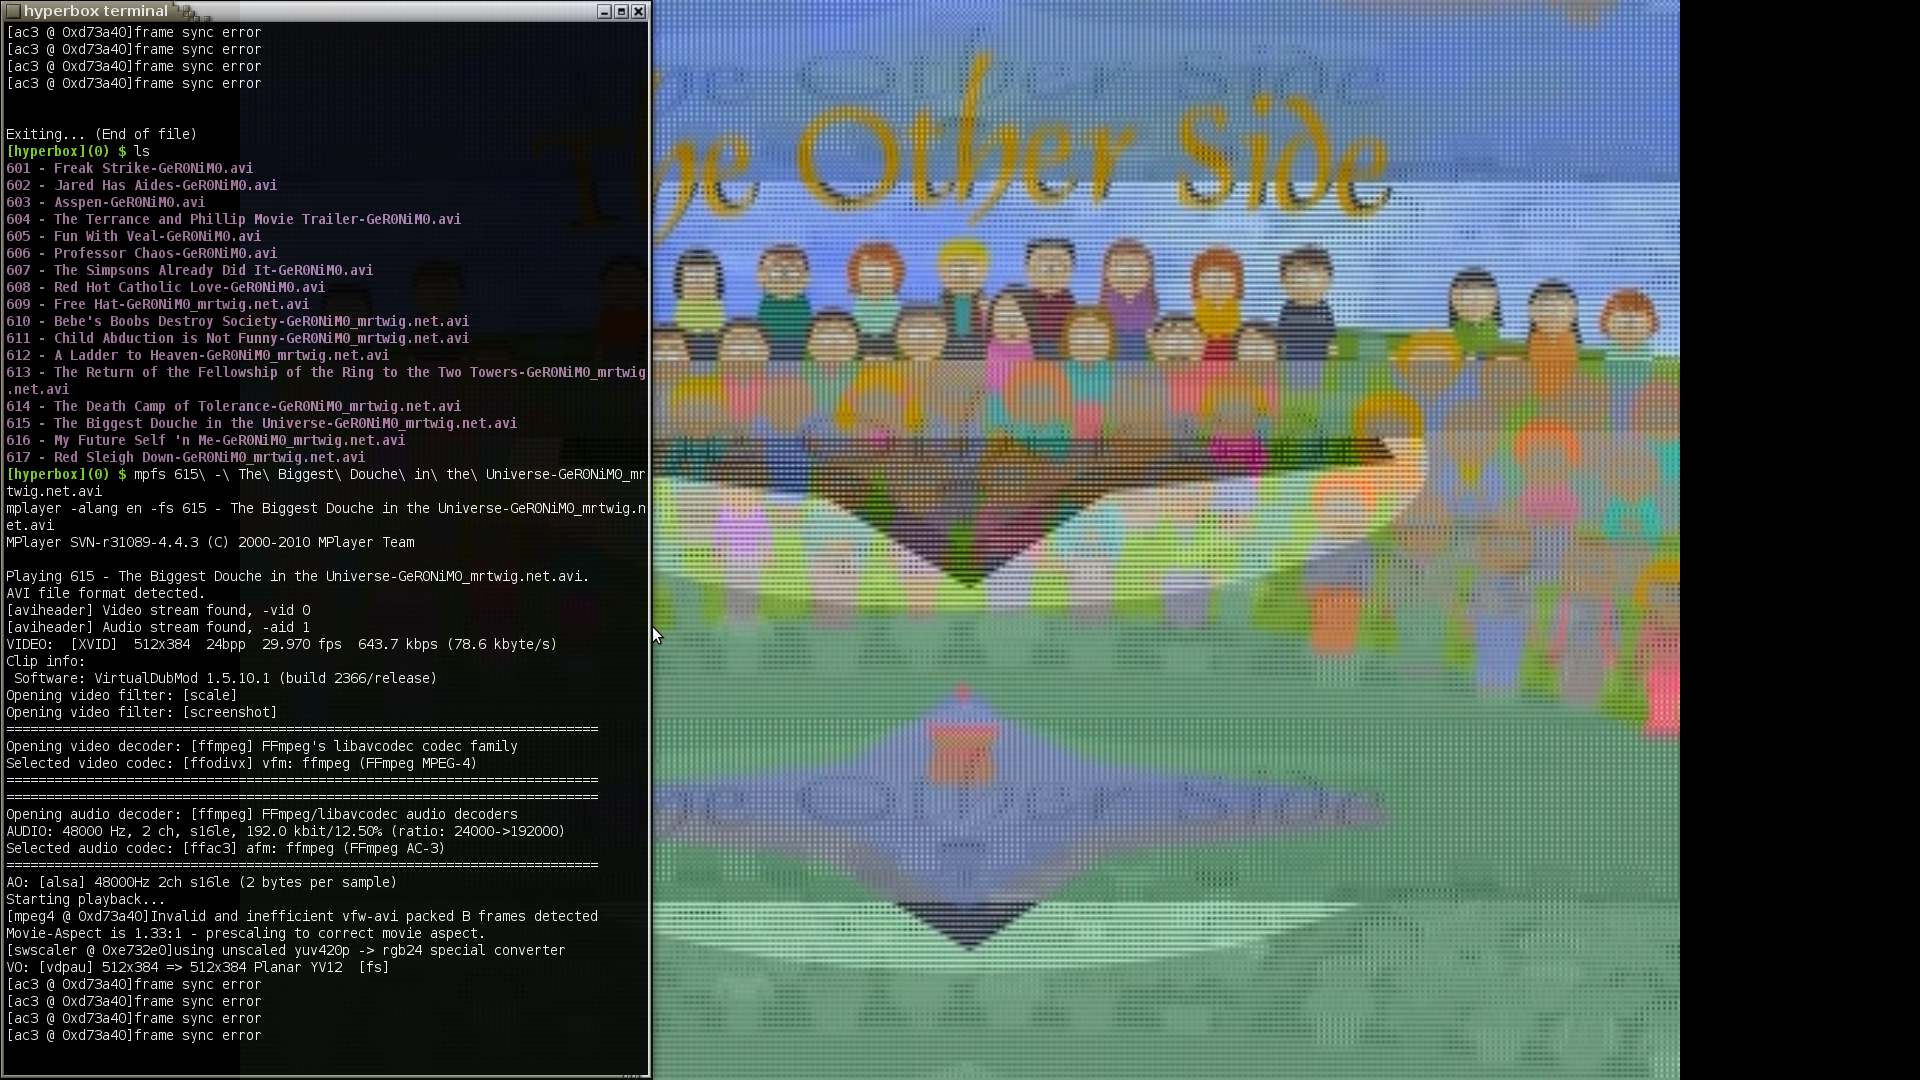
\includegraphics[width=4cm]{texobjs/shitfuckedup.png}
}
\end{figurehere}
%%%%%
\begin{comment}
One of the possibilities we investigated was whether an arbitrary CUDA kernel would be able 
to modify the system's video channel.  The threat model we considered was arbitrary code
being able to manipulate the video channel.  

In one case, this could consist of grabbing the current 
framebuffer to obtain information from other programs.  In another case, this could consist of modifying the 
current framebuffer in an effort to deceive the user into believing the system is in a different state than 
it actually is.  For example, if one could replace the padlock icon
commonly used on browsers to indicate a secure web connection, an attacker could fool a user into believing 
that they have a secure and authentic connection when in fact they do not.

The memory that CUDA code can access consists of three types: per-thread local memory, 
per-block shared memory, and global memory.  However, this memory differs from the framebuffer 
that is used by the graphics card to update the display.  We analyzed the possibility of both reading 
and writing to the framebuffer in the case of CUDA applications.

We first examined the case of reading the current framebuffer.  Not only is this necessary in order 
to be able to modify it, but it can lead to information disclosure as well.  While CUDA provides several 
methods for obtaining the current framebuffer, all of these methods rely on interfacing with OpenGL or Direct3D 
through the provided interfaces.  

In the case of OpenGL, glReadPixels() can be used to obtain the current framebuffer.  
While this can be done within a CUDA program, it is not done using CUDA itself.  The data can be pulled into CUDA directly 
via several methods, including the use of cudaGraphicsMapResources or cudaGLMapBufferObject\cite{cudaguide}\cite{cudareference}.  In this instance, CUDA provides no added benefit or significant difference over existing programs.

Similarly, writing to the framebuffer is not explicitely possible in CUDA, and similar methods must be used as to read from it (i.e. using OpenGL or Direct3D within CUDA).

However, CUDA provides both read and write access to video memory, and the framebuffer is contained within memory.  Unfortunately, our tests were unsuccessful at locating the location of the framebuffer in memory.  This indicates either that the CUDA API disallows access to the region of memory containing the framebuffer or that there is a system in place that provides a hardware barrier between the framebuffer and the rest of VRAM for this purpose.

%WTF happened on my system - artifacting.  Could this be exploited somehow?%
While we were unable to specifically locate the framebuffer in memory, during our tests we did encounter several cases of video artifacting on our displays.  This led us to believe that there must be some method of accessing the framebuffer by using CUDA in a way that it was not intended for.  As of the writing of this paper we have been unable to isolate the circumstances that led to the artifacting and to reproduce them in a controlled manner, but we believe there is promise in future work being done in this area.

%Hopefully the above section can be updated, but as of now I have no clue what happened on my system to produce the artifacting.  I'll take another look at it but it'll probably have to wait until after my take-home final is done%
\end{comment}

\section{Defending CUDA}
Implementors of competing CUDA stacks must ensure that their systems implement
the relatively successful memory protections extant in the NVIDIA solution. The
following properties ought be considered in designs, and verified:
\squishlist
\item CUDA manifests a Harvard architecture atop what is likely a Von Neumann
unified memory. It is necessary that code be properly protected, especially
under Compute Capability 2.0's concurrent kernels.
\item CUDA performs memory translation and protection, almost certainly in
hardware. It is necessary that these mechanisms be properly configured,
and that proper invalidations are performed in the face of remappings. Concurrent
kernels must not be able to freely read each other's memory.
\item CUDA monitors processes from within kernelspace, freeing their device
resources on termination. This must be duplicated, and must be performed in
kernelspace to be effective.
\item It ought be ensured that device control maps are not shared with device
code via a secondary mapping. This code must be located in kernelspace.
\item It would be valuable for CUDA to make available more forensic information.
In particular, the standard UNIX process accounting mechanism ought be honored.
Furthermore, rate-limiting ought use the standard, configurable klogd policies.
\item CUDA resources ought be accounted for by the \texttt{rlimit} infrastructure.
It is absolutely critical that this be done for mapped host memory.
\squishend

% do we really want this?
\begin{comment}
\section{Related work}
Our research in this area is focused on the possibility of security
vulnerabilities against the GPU itself, an area which we were unable to find
prior research for. However, our research is motivated in part by an increase
in applications being developed for GPUs and also by GPUs being used as the
processing unit for security related tasks.
  
\subsection{General applications}
  
  Dedicated graphical processing units (GPUs) have seen significant advancement
in the past couple decades due to the insatiable demand that consumers have for
ever-increasing advances in video game graphics. This development has led to
recent GPUs reaching the point where they are powerful enough that there has
been significant research invested into using them to execute tasks outside the
realm of video games. One of the most popular examples of this is the
Folding@Home project, which in recent years has developed a version of its
application that runs on both ATI and NVIDIA brand GPUs\cite{foldingathome}.
  
  In 2007, NVIDIA released an SDK for CUDA, their ``Compute Unified Device
Architecture'', allowing for the GPU to be much more accessible to developers
wishing to use the GPU for non-graphical applications. In the three years since
then, a wide variety of applications for CUDA have been developed\footnote{\url{http://www.nvidia.com/object/what\_is\_cuda\_new.html}}.
  
  General Mills developed an application that used CUDA to model the optimal
way to cook a frozen pizza in a microwave. SeismicCity used CUDA to improve the
amount of time it takes to interpret seismic data to determine the optimal
drilling locations for finding oil\cite{cudainaction}.
  
  Other companies are offering CUDA solutions for problems in the realms of
electromagnetics, bioinformatics, finance, accelerator physics, aerodynamics,
engine optimizations, image and video stream compression, healthcare and life
sciences, medical imaging, defense, and more\footnote{For a full list, see \url{http://www.nvidia.com/object/cuda\_in\_action.html}}.
  
\subsection{Security-related computation}
  There are a few research areas where GPUs have been used in security applications, but all of these involve using the GPU as a faster processor than the CPU, and none of the research involves investigating the GPU itself or coding frameworks such as CUDA from a security standpoint.
  
  The most common security task that GPUs have been used for in prior work have been to use the GPU for performing cryptographic computations. Research has found that GPUs can perform some AES-related OpenSSL computations up to 20 times as fast as a typical implementation
\cite{cudaaes}. Another aspect that is of importance, particularly to copyright groups such as the RIAA and MPAA, are the encryption techniques used with GPUs for the security of applications involving remote displays, such as for HDCP blu-ray implementations\cite{cryptographics}.
  
  While GPUs can be used for improving the speed of cipher implementations, they can be used to speed up cryptographic attacks as well. In some cases, applications have been developed using CUDA to allow for WiFi keys to be broken up to 100 times as fast as in typical implementations \footnote{\url{http://www.elcomsoft.com/edpr.html}}.
  
  Intrusion detection systems can exhibit performance degradation under heavy
  loads, and some of the proposed solutions to this problem have involved
  offloading IDS computations to the GPU
  \cite{offloadids}.
  Additionally, some techniques in pattern-matching are difficult to perform
  quickly enough to be useful, and GPUs have been proposed as a solution that
  allow for significant decreases in computation time
  \cite{gpuids}.

\end{comment}

 \section{Conclusions} 
The recommendations of the Orange Book\cite{orangebook}, requirements of the Common Criteria\cite{ccrit},
and animadversions of Saltzer and Schroeder\cite{principles} have long provided general principles for
security-conscious design. These principles have been at least superficially
observed along the way to NVIDIA's CUDA system. Reverse engineering of the
CUDA software stack and validation of open-source competition will reveal how
truly sound the implementations may be. Modern GPUs are some of the world's most powerful devices. Harnessing these
mighty processing units is necessary to even approach full machine utilization.
This will become only more true:
\begin{itemize}
\item Increasing the clock frequency affects cooling and power requirements
(dynamic power consumption is proportional to frequency). Furthermore,
clock frequency increases tend to force decomposition of pipeline
stages, exacerbating branch misprediction delays and pressuring any OOO
system\cite{cormean}.
\item Increasing the issue width, or duplicating functional units, either
requires ISA changes (for VLIW) or massive frontend resources for lookahead,
disambiguation, and hazard tracking. Assuming these expenses acceptable,
diminishing returns result from limitations of instruction-level parallelism.
Furthermore, very wide issues lead to sparse code flows, taxing the instruction
store subsystem. 
\item Further investments in cache --- and thus, hopefully, fewer memory
delays --- serve only to approach more closely a device's theoretical peak.
That peak itself is a function of architecture, not of programs or their
access patterns.
\item Investments in OOO apparatus (reorder buffers,
frontend reservation stations, register renaming) yield diminishing returns due
to the profound limitations of instruction level parallelism\cite{phenn}. Like improvements
to cache, OOO can only hide delays, not find new FLOPS\@.
\item Denser chip-multithreading similarly serves only to hide latency.
\item Larger chips require either pipelined wires or high voltages to operate
reliably, and place strict requirements on clock-signaling circuity. Efficient
power management requires complex and expensive partial power gating\footnote{For
instance, feeding $\mu$ops from Nehalem's Loop Stream Detector results in power-down
of the leading three pipeline stages.}.
\end{itemize}
We see that FLOPS --- at any price --- can be had only by adding cores or extending
SIMD order. The former is obviously easier with small, in-order, SISD cores,
such as the unified shaders of a modern GPU\@; duplicating a Nehalem core is a
much more daunting process. As for the latter, note that Intel's ``Sandy
Bridge'' microarchitecture is expected to add the AVX instruction scheme and
its 256-bit \texttt{YMM} vector registers\cite{avx}\cite{fma4}. The data-based decomposition of CUDA's
``SIMT'' model can immediately take advantage of their new cores (given
sufficiently large problem sets, of course), whereas x86 binaries\footnote{Most of them, anyway.} would
require dynamic translation or recompilation to take advantage of the new SIMD
order.

Extensive manycoring and huge memory bandwidths are certainly the key to FLOPS.
Without security-conscious analysis and verification of infrastructure and
policy, they must not be trusted in a multiprocessing context. As GPUs become
more and more general-purpose, the attack space will grow; Compute Capability 2.0
already adds significant complexity and danger. The only answer is constant
vigilance.
\bibliographystyle{acm}
\bibliography{cs8803ssProject}
\end{multicols}
\appendix
\newpage
\section{\texttt{strace(2)d} CUDA binary}\label{strace}
\VerbatimInput[fontsize=\scriptsize,numbers=left,framerule=.8mm,label=strace(2)d deviceQueryDrv]{texobjs/deviceQueryDrv.strace}
\newpage
\section{\texttt{libcuda.so.195.36.15} 3.0 symbols}\label{strace}
\VerbatimInput[fontsize=\scriptsize,numbers=left,framerule=.8mm,label=dynamic symbols]{texobjs/cudasymbols}
\section{\texttt{dmesg} output from hung task}\label{oops}
\VerbatimInput[fontsize=\scriptsize,numbers=left,framerule=.8mm,label=dmesg]{texobjs/crash}
\section{\texttt{dmesg} output from wayward OOM killer}\label{oops}
\VerbatimInput[fontsize=\scriptsize,numbers=left,framerule=.8mm,label=dmesg]{texobjs/oom}
\end{document}
